
% \section{Backend}
% \label{sec:Backend}

% TODO move to marco teorico

El backend de la aplicación comprende el manejo de la información y cómo es procesada para su consumo por parte del frontend y almacenamiento en la base de datos, por lo tanto se pueden observar dentro del backend, 2 secciones claramente diferenciadas: el servidor web y la base de datos.\\




\subsection{Servidor Web}
\label{sub:servidor_web}

Un servidor web se puede referir a 2 cosas, la primera es la máquina en la cual se instalará y alojara toda la lógica de negocio que requiere la aplicación, la segunda se refiere a la capacidad de poder recibir y dar información al cliente del servidor, el segundo caso es también conocido como un \emph{servicio web} el cual será discutido en esta sección.\\

El servidor web es el encargado de enviar la página HTML la primera vez que el cliente hace un request al servidor, una vez que la página está cargada el servidor solo se encarga de enviar y recibir información de la base de datos al cliente.\\

El servidor web será construido con \emph{Express JS}, para lo cual primeramente se necesita instalar \emph{Node JS}, \emph{Express JS} cuenta con una herramienta para la consola, \emph{express-generator}, entonces solo es necesario crear un projecto Express y empezar a implementar la lógica de negocio.\\

El servidor se va a encargar de hablar con la base de datos y también necesita ofrecer una interfaz por la cual pueda recibir datos y entregar datos, en pocas palabras un \emph{API}, implementar un \emph{API} con \emph{Express} es bastante sencillo, para trabajar con la base de datos se instaló una librería \emph{BookshelfJS} para poder escribir las consultas y trabajar con la base de datos como si se tratara de objetos, este patrón se denomina \emph{ORM} o \emph{Object-Relational-Model}, básicamente mapea las tablas y las relaciones existentes como objetos dentro del paradigma \emph{OOP} y el framework se encarga de traducirlo a lenguaje \emph{SQL} que es el lenguaje que entienden las bases de datos, \emph{BookshelfJS} también permite escribir las consultas en lenguaje \emph{SQL} si fuera necesario, como en el presente caso ya que al  trabajar con una herramienta específica, \emph{pgRouting}, las consultas son personalizadas.\\

% \begin{minted}{js}
 \begin{center}
   \begin{verbatim}
     var getPlace = (req, res) => {
       var id = req.params.id;
       var raw = "SELECT " +
                 " ST_AsGeoJSON(geom)::json As geometry," +
                 " name," +
                 " description," +
                 " phone," +
                 " level," +
                 " gid As id " +
                 " FROM place WHERE gid = " + id;
       Bookshelf.knex.raw(raw)
         .then((data) => {
           res.json(data.rows[0]);
       })
         .catch((error) => {
           console.log(error);
           res.send("Error");
       });
     };
   \end{verbatim}
 \end{center}
 %  \end{minted}

Como en la anterior consulta, se requiere obtener la información de un lugar, por lo tanto se necesita  usar la forma \emph{Raw SQL} o consultas en ``SQL puro'' ya que el fuerte de \emph{BookshelfJS} es el manejo de las consultas en forma de objetos (ORM), lamentablemente actualmente no existe mucho soporte para manejar datos geoespaciales por parte de frameworks ORM.\\

% De esta forma se obtiene de la base de datos la infor  donde este
Una vez que se obtiene la información del lugar; nombre, descripcion, telefono, el nivel o piso, pero lo importante de esta consulta es la obtención del ``punto'' geoespacial del lugar. Estos datos son importantes para implementar la lógica de negocio.\\


\begin{center}
 \begin{verbatim}
   "POINT (-66.14857015827988 -17.394421906929086)"
 \end{verbatim}
\end{center}

% var raw = "SELECT seq, id1 AS node, id2 AS edge, cost
%            FROM pgr_dijkstra('SELECT gid AS id,
%                                     source::integer,
%                                     target::integer,
%                                     st_length(geom) AS cost
%                               FROM public.ways', targetId, sourceId, false, false);";


Este atributo es de tipo \emph{punto} o \emph{point} el cual tiene un \emph{SRID} o \emph{Spatial Reference System Identifier}, el \emph{SRID} corresponde a un sistema de referencia espacial basado en el elipsoide concreto usado para la creación de mapas de tierra plana o de tierra redonda.\cite{msdn_srid}\\

El \emph{SRID 3857} también conocido como \emph{EPSG 3857} es la implementada en la \emph{Proyección de Mercator}, el SRID  es la llave primaria de la tabla \emph{spatial\_ref\_sys} que se crea cuando se inicializa \emph{PostGis} en una base de datos para que esta soporte información geoespacial, esta tabla provee la información necesaria para interpretar y convertir correctamente todas las coordenadas existentes, el \emph{SRID 3857} está definida en la tabla \emph{spatial\_ref\_sys} como ``Popular Visualisation CRS / Mercator''.\\

En resumen el servidor web será el encargado de recibir información y devolver una respuesta de acuerdo a los datos que recupere de la base de datos, para tal efecto se utilizan las direcciones URL, las cuales de acuerdo al protocolo HTTP se pueden definir de acuerdo a la acción que el servidor necesita procesar, para lograr esta comunicación es necesario definir nuestro API.\\
% TODO move to marco teorico




% movido a iteracion 1
\subsubsection{Implementación del REST API}
\label{subs:Implementacion del REST API}



El servidor necesita reconocer las peticiones que le llegan del cliente, para lo cual es necesario ``mapear'' un URI a una acción específica, las cuales ya están preparadas para comunicarse con la base de datos, no hay restricción en la declaración de las URIs pero para una mejor comprensión del API que se está desarrollando es necesario seguir convenciones que aseguran que cualquier desarrollador pueda comprender el API presentado y pueda ser fácilmente consumido por cualquier aplicación que requiera acceder a la información que disponible, un API REST es el que cumple con estas características.
En primer lugar es necesario crear las URIs que serán ``entendidas'' por el servidor, esto se logra declarando en el servicio creado con \emph{Express.JS}, tal como se puede apreciar en el siguiente bloque de código, cada URI se lo relaciona a un modelo en específico de acuerdo a la acción que se requiere, tal como se puede observar en el cuadro \ref{tab:rest} las URIs declaradas en el API cumplen con tal característica.\\


% \begin{minted}{js}[label=express_api,caption=Declarando API REST con ExpressJS]
\begin{center}
  \begin{lstlisting}[label=express_api,caption=Declarando API REST con ExpressJS]
        const router = express.Router();
        router.get('/', places.getAll);
        router.get('/:id', places.getPlace);
        router.post('/', places.newPlace);
        router.put('/:id', places.editPlace);
        router.delete('/:id', places.deletePlace);

        app.use('/api/v1/places', router);
  \end{lstlisting}
\end{center}
% \end{minted}

% En el código

  %
  % Para lograr todo este comportamiento  es necesario declarar, en el archivo
  % que controla las rutas dentro de la aplicación, \textbf{routes}, que el
  % recurso \textbf{user} es \emph{restful}, tal como se muestra en la figura \ref{fig:rest}\\

  % \begin{figure}[!hbp]
  %   \begin{center}
  %     \caption[REST - routes.rb]{config/routes.rb}
  %     \label{fig:rest}
  %     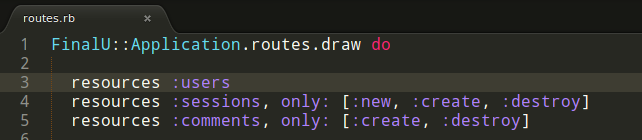
\includegraphics[width=1\textwidth]{rest}
  %     \caption*{Fuente: }
  %   \end{center}
  % \end{figure}

  El cuadro \ref{tab:rest} muestra como se puede leer las peticiones al API de \textbf{places}, las acciones mostradas son las que se pueden encontrar en un API REST pero no es necesario declararlas todas para considerar a que un API es restful.\\


  \begin{table}[!hbp]
    \begin{center}

      \begin{tabularx}{0.75\textwidth}{ l l l  X }
        \toprule
        \multicolumn{1}{c}{\textbf{HTTP}} &
        \multicolumn{1}{c}{\textbf{URI}}  &
        % \multicolumn{1}{c}{\textbf{C}}  &
        \multicolumn{1}{c}{\textbf{ACCI\'ON}} &
        \multicolumn{1}{c}{\textbf{USADO PARA}}  \\
        \multicolumn{1}{c}{\textbf{request}} & & & \\

        \midrule
        GET     &  /places    &  index    & devuelve una lista con todos los lugares\\
        POST    &  /places    &  create   & inserta un nuevo lugar en la bd\\
        GET     &  /places/1  &  show     & muestra el lugar con identificador \emph{1}\\
        PUT     &  /places/1  &  update   & actualiza los datos de un lugar específico\\
        DELETE  &  /places/1  &  delete   & elimina el lugar con id = 1 de la bd\\
        \bottomrule
      \end{tabularx}

      \caption[recursos REST]{REST URIs para los lugares}
      \label{tab:rest}

      \caption*{Fuente: Elaboración propia}
    \end{center}
  \end{table}

  % Tal como se ve en el cuadro \ref{tab:rest}, Rails maneja los request HTTP de acuerdo con
  % el tipo de llamada que se realice, este trabajo lo realiza el \textbf{router},
  % que reconoce las URLs y los despacha a una \textbf{acción} del controlador,
  % todo este proceso ya está implementado en el núcleo de Rails por lo tanto  es automático y el programador
  % no necesita más configuración que la mostrada en la figura \ref{fig:rest},
  % obedeciendo al principio de \emph{Convención sobre configuración}\\

  % % no son más que métodos dentro del \emph{user\_controller.rb}
  % el cual
  % es parte del controlador de la arquitectura MVC.\\

  % The Rails router recognizes URLs and dispatches them to a controller’s action. It can also generate paths and URLs, avoiding the need to hardcode strings in your views.

  Por ejemplo, si se genera una petición GET hacia la direcci\'on
  \mbox{\emph{/places/1}}  el servidor interpreta la dirección y responde
  mostrando la información del lugar “1” y en cambio si se genera
  una petición PUT a la misma direcci\'on \emph{/places/1} se ejecuta la acción \textbf{update} y se actualizan los datos del lugar ``1''.

  % \textbf{usuarios} actualizando la información del usuario “1”. \\

  Siguiendo la convención de un API REST ayuda a entender el flujo que tiene un recurso,
  las URL son legibles y únicos para cada recurso. Por lo tanto la implementación   de los recursos se hace de forma más limpia y ordenada, situaciones que son   claves para el mantenimiento y la extensibilidad del sistema.
% movido a iteracion 1


% TODO move to marco teorico
\subsection{La Base de Datos}
\label{sub:data_base}

     %
     % \subsection{Que se us\'o en la Aplicaci\'on} % (fold)
     % \label{sub:que_se_uso_en_la_aplicacion}
        Para preparar la base de datos es importante entender las diferencias entre los distintos tipos de sistemas de coordenadas porque computacionalmente realizar operaciones sobre los sistemas de coordenadas tiene un costo.\\

       Si se usara el sistema de coordenadas geográfico (WSG84) este es el más apropiado si se necesitaría usar grandes extensiones de la superficie terrestre, que al ser una estructura elipsoidal el costo computacional para realizar las operaciones matemáticas de calcular distancias, intersecciones, etc. es más elevado. En cambio el uso de un sistema de coordenadas proyectado (Mercator Projection) tiene un costo computacional más bajo, ya que se estaría trabajando con un sistema geométrico.\\

       % Por otro lado,
       También hay tomar en cuenta la base de datos, ya que será esta la que se encargará de manejar los datos espaciales. Al estar usando PostGIS, se puede ver que en su documentación que claramente exhorta el uso de un sistema geométrico sobre el uso de un sistema geográfico si  se va trabajar con datos que cubran una pequeña área geográfica. Tomando en cuenta esta recomendación y el tamaño del área de estudio (el campus de la UMSS), se procedió a implementar en la base de datos el uso de la proyección Mercator. Se va usar Mercator sobre las otras proyecciones porque aparte de las ventajas que se mencionaron con anterioridad, Google Maps usa esta proyección y ya que se usará este mapa lo más correcto es trabajar con la misma proyección. \\

% \footnote{ http://postgis.org/documentation/manual-1.5/ch04.html} documentacion Postgis

       Toda la información geoespacial recolectada necesariamente debe ser almacenada, para lo cual se investigó las diferentes bases de datos disponibles y tras la tarea de investigar acerca de ese problema se procede a instalar \emph{PostgreSQL 9.4.8} sobre Linux \emph{Ubuntu 15.10}, y para manejar datos geoespaciales se necesitó instalar \emph{PostGIS 2.1.8}.\\
% TODO move to marco teorico

% movido a iteracion 1
       \subsubsection{Los lugares}
       \label{subs:Los lugares}

       En primer lugar se recolectó la información de los lugares, que la aplicación contendrá  de forma inicial, al igual que para recolectar las rutas se hizo uso de un \emph{GPS Garmin Nuvi 1300}, el cual cuenta con la opción de guardar locaciones como favoritos, entonces solo fue necesario estar cerca del lugar que se desea guardar y activar esa opción del GPS, este guarda la información en un archivo \emph{.gpx} y con la ayuda de \emph{QGIS} se genero el archivo shapefile correspondiente.\\

       Posteriormente es necesario pasar la información geoespacial del shapefile a la base de datos, para esta tarea se hizo uso de una herramienta disponible para postgres, \emph{shp2pgsql}, que permite la conversión de un archivo shapefile a un archivo sql.

       % $ shp2pgsql -s 4326 -I -S -c -d ~/Documents/places.shp > places.sql
       \begin{verbatim}
         $ shp2pgsql -s 3785 -I -S -c -d ~/Documents/places.shp > places.sql
       \end{verbatim}

       Con el anterior comando se tiene como resultado un archivo \emph{.sql}, el cual es ingresado en la base de datos ya configurada, de esta forma nuestra base de datos para a contener una tabla geoespacial con datos de tipo \emph{POINT}, los cuales representan los lugares dentro del campus de la UMSS.\\

       % \begin{verbatim}
       %   $ shp2pgsql -s 4326 -I -S -c -d ~/Documents/ways.shp > ways.sql
       % \end{verbatim}
       %
       % De la misma forma es necesario pasar la información de las rutas contenidas en un archivo shapefile a un archivo sql, en este caso creará una tabla \emph{WAYS}.\\

       El archivo \emph{sql} resultante es usado para popular la base de datos con la información inicial de los lugares que contiene el campus universitario, para tal tarea se usó el siguiente comando.\\
       % Los archivos resultantes \emph{sql} son usados para popular la base de datos .\\

       \begin{verbatim}
         $ psql -d db_ubikate -U db_admin -f /Documents/places.sql
       \end{verbatim}

       \begin{figure}[H]
         \begin{center}
           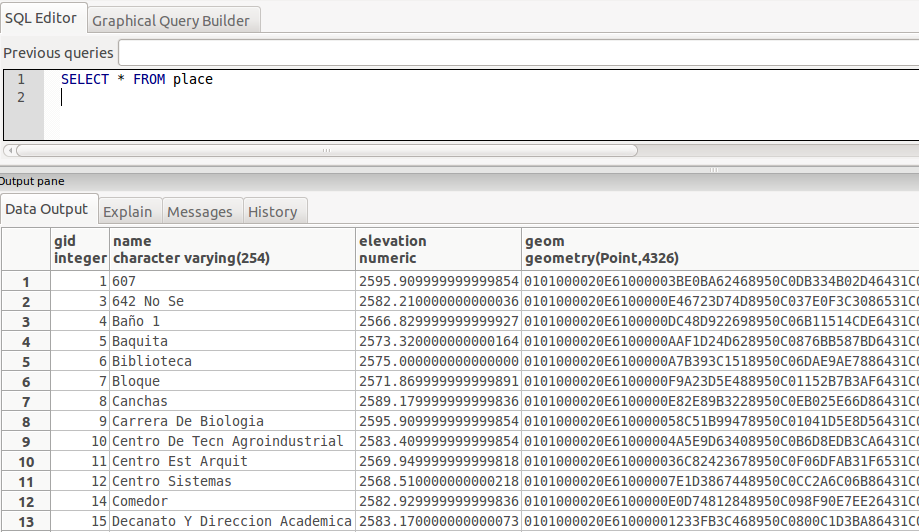
\includegraphics[width=1\textwidth]{iteration1/postgres_places}
           \caption{Herramienta gráfica de PostgreSQL (\emph{pgAdmin}).}
           \label{fig:postgres_places}
           \caption*{Fuente: Elaboración propia}
         \end{center}
       \end{figure}
        % con la tabla de Lugares desplegada.

       En la figura \ref{fig:postgres_places} se puede observar que la columna \emph{Elevation} contiene datos que el GPS Garmin Nuvi 1300 genera al momento de guardar un punto, en el presente caso es irrelevante.\\
% movido a iteracion 1


% movido a iteracion 2

       \subsubsection{Las Rutas}
       \label{subs:Las Rutas}

       Después de generar un archivo shapefile en la sección \ref{sec:generar_mapa_rutas}, se procede a popular la base de datos del mismo modo que se hizo con la información de los lugares. Para las rutas se genera una tabla nombrada \emph{ways}.\\

       Posteriormente se procede a preparar la tabla \emph{ways} para que soporte las funciones instaladas por pgRouting.
       % Una vez poblada la base de datos se procede a cargar la misma con la información obtenida en RF011, para tal efecto es necesario primeramente crear una tabla que contendrá los LINESTRING contenidos en el shapefile, esta operación es similar a la realizada en la tarea - RF003 (\ref{sub:RF003}). Una vez que ya se tiene la tabla a la llamamos \emph{ways},
       Es necesario ejecutar un query propio de \emph{pgRouting} el cual tiene como objetivo analizar los datos geo-espaciales de la tabla y añadirle una \emph{topología}.\\

       \begin{verbatim}
         select pgr_createTopology('ways', 0.00000001, 'geom', 'gid');
       \end{verbatim}

       Dentro lo que es la \emph{topología geoespacial} existe una aplicación que se lo conoce como \emph{topología de red}. La \emph{topología de red} representa las relaciones entre segmentos en una red lineal o una colección de segmentos de línea. \cite{osgeo_journal_topology} \\

       En un \emph{SIG} la topología ayuda a mejorar el análisis de datos geo-espaciales, para resolver el problema de la ruta corta \emph{pgRouting} genera una \emph{topología de red} usando los datos que existen en la tabla \emph{ways}, es necesario ejecutar una instrucción, la que se muestra a continuación y \emph{pgRouting} se encarga de llenar los datos que se pueden observar en la figura \ref{fig:postgres_ways}, las columnas \emph{source} y \emph{target} son populadas con el análisis topológico y en la figura \ref{fig:postgres_vertices}, se puede observar que la tabla \emph{ways\_vertices\_pgr} es creada enteramente en la ejecución de la instrucción.\\

       \begin{figure}[H]
         \begin{center}
           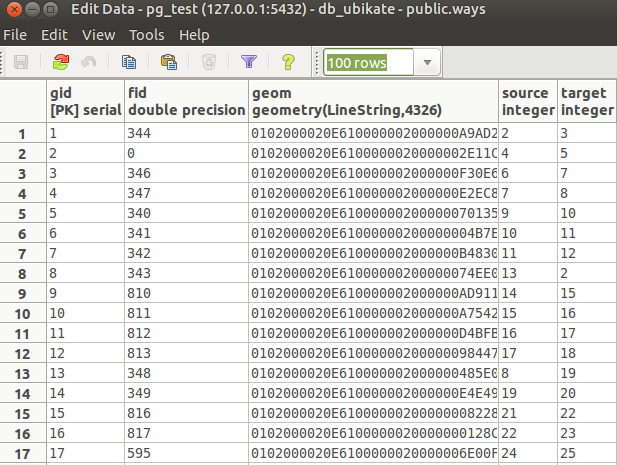
\includegraphics[width=1\textwidth]{iteration2/postgres_ways}
           \caption{Vista de la tabla \emph{ways}.}
           \label{fig:postgres_ways}
           \caption*{Fuente: Elaboración propia}
         \end{center}
       \end{figure}

       En la figura \ref{fig:postgres_ways} se puede apreciar que cada fila es una parte de la línea original obtenida por el dispositivo GPS y explosionada por QGIS, hay que notar que las columnas \emph{source} y \emph{target} hacen referencia a los nodos o vértices que la primera línea tiene en sus extremos, la primera línea o fila está identificada por la columna \emph{gid}.\\

       En la siguiente figura \ref{fig:postgres_vertices} se observa la tabla \emph{ways\_vertices\_pgr} que contiene los vértices creados a partir del análisis de los datos en la tabla \emph{ways}.

       \begin{figure}[H]
         \begin{center}
           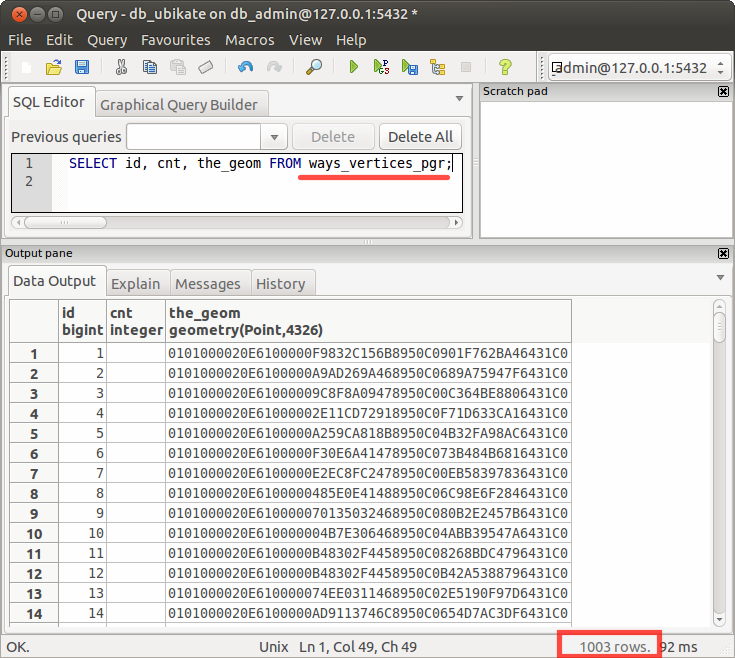
\includegraphics[width=1\textwidth]{iteration2/postgres_vertices}
           \caption{Vista de la tabla \emph{ways\_vertices\_pgr}.}
           \label{fig:postgres_vertices}
           \caption*{Fuente: Elaboración propia}
         \end{center}
       \end{figure}

       Para entender los datos generados hay leer la información de las 2 tablas, por ejemplo en la primera  fila (gid 1) de la tabla \emph{ways}, se observa que el contenido de la columna \emph{source} es igual a \textbf{2} y \emph{target} es igual a \textbf{3}, eso quiere decir que los vértices del LINESTRING de la fila 1 son los vértices con \textbf{id} 2 y 3 respectivamente de la tabla \emph{ways\_vertices\_pgr}.\\


       Todo el conjunto de vértices y líneas de estas tablas se podría representar con una Matriz de adyacencias, explicada en \ref{sub:representacion_de_un_grafo}, y usada en la resolución de la ruta mas corta, mas específicamente con el algoritmo de Dijkstra.\\

       \begin{center}
         \begin{lstlisting}[label=pgr_dijkstra,caption=Algoritmo de Dijkstra implementado en \emph{pRouting}]
           SELECT seq, id1 AS node, id2 AS edge, cost
           FROM pgr_dijkstra(SELECT gid AS id,
                                     source::integer,
                                     target::integer,
                                     st_length(geom) AS cost
                              FROM public.ways, targetId, sourceId, false, false);
         \end{lstlisting}
       \end{center}


       La anterior consulta SQL es una llamada al método \emph{pgr\_dijkstra} implementado en \emph{pgRouting} el cual solo puede ser utilizado una vez que la base de datos está preparada para tal efecto, es decir necesitamos que la tabla de rutas \emph{ways} tenga la topología de red y también es necesario los ids de los nodos de destino y origen, \emph{targetId} y \emph{sourceId} respectivamente, estos dos últimos datos son obtenidos por una combinación de acciones ya que los nodos son propios del mapa de rutas y el punto destino es en realidad un lugar el cual está ubicado en otra tabla y el punto origen es donde se encuentra el cliente dentro del campus Universitario, por lo tanto una vez obtenido los punto geo-referenciados del lugar de la tabla \emph{places} y el punto donde se encuentra parado el cliente se obtienen los nodos ``más'' cercanos a estos puntos, gracias a que \emph{PostGIS} ya lo tiene implementado, encontrar el nodo más cercano es tan fácil como ejecutar la siguiente consulta SQL, donde \emph{lon} y \emph{lat} son la longitud y latitud del lugar.

       \begin{verbatim}
           SELECT id
           FROM ways_vertices_pgr
           ORDER BY the_geom <-> ST_GeometryFromText('POINT(lon lat)', 4326)
           LIMIT 1
       \end{verbatim}

       Una vez ejecutado el método \emph{pgr\_dijkstra} se obtiene un conjunto de líneas, que son un conjunto de latitudes y longitudes que representa la ruta más corta entre el punto origen y el punto destino, esta información realmente no dice nada a la persona que lo lee por lo tanto requiere ser procesada para poder ser consumida desde el navegador, este proceso es llevada a cabo en el servidor y entregada al cliente en formato GeoJSON.\\
 % movido a iteracion 2


       % En la figura XX, se puede ver la tabla \emph{WAYS} con las rutas generadas.





       % Como projected
       % PostGIS maneja dos tipos de datos, geográficos y geométricos

     % section que_se_uso_en_la_aplicacion (end)
 % section sistema_de_coordenadas_para_datos_geograficos (end)
 % \section{Tipo de archivos} % (fold)
 % \label{sec:tipo_de_archivos}
 %
 % section tipo_de_archivos (end)

 % \subsection{Implementaci\'on} % (fold)
 % \label{sub:Implementacion}


   % Para manejar datos georreferenciados con tecnología JavaScript, ya que se implementó el Backend con NodeJS, se hizo uso de la librería \textbf{KnexJS} para manejar la conexión a la base de datos PostgreSQL, y BookshelfJS para las consultas SQL pero para las consultas con datos geoespaciales se realizó a través de esta herramienta pero usando la forma \emph{Raw SQL}\footnote{Raw SQL se refiere a consultas en ``SQL puro'' ya que el fuerte de BookshelfJS es el manejo de las consultas en forma de objetos (ORM), lamentablemente actualmente no existe mucho soporte para manejar datos geoespaciales}.


% Para implementar la comunicación con la base de datos se

% El proyecto

% La estructura de archivos dentro del proyecto \emph{Express} se puede observar en la figura \ref{fig:express_structure}, donde se puede observar las secciones principales de routing, que se encarga de direccionar las peticiones web de acuerdo del protocolo HTTP, la sección de \emph{views} dónde están los templates

% \begin{figure}[H]
%   \begin{center}
%     \caption[Express Application Structure]{Estructura de archivos de una Aplicación \emph{Express}}
%     \label{fig:express_structure}
%     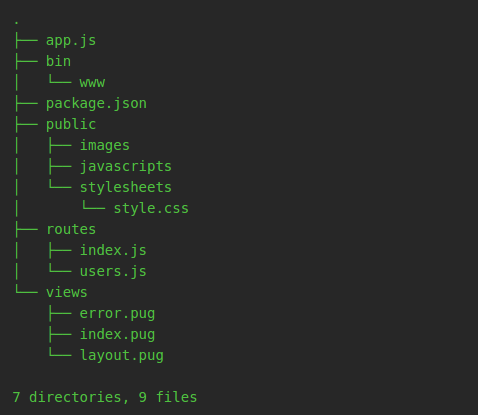
\includegraphics[width=1\textwidth]{express_structure}
%     \caption*{Fuente: https://expressjs.com}
%   \end{center}
% \end{figure}

% Dentro del proyecto \emph{Express} definimos una sección donde localizamos la conexión y las consultas a la base de datos, y otra sección donde



 %
 % Para manejar datos georreferenciados con tecnología JavaScript, ya que se implementó el Backend con NodeJS, se hizo uso de la librería \textbf{KnexJS} para manejar la conexión a la base de datos PostgreSQL, y BookshelfJS para las consultas SQL pero para las consultas con datos geoespaciales se realizó a través de esta herramienta pero usando la forma \emph{Raw SQL}\footnote{Raw SQL se refiere a consultas en ``SQL puro'' ya que el fuerte de BookshelfJS es el manejo de las consultas en forma de objetos (ORM), lamentablemente actualmente no existe mucho soporte para manejar datos geoespaciales}.
 %
 % \begin{center}
 %   \begin{verbatim}
 %     var raw = "SELECT " +
 %                 " ST_AsGeoJSON(geom)::json As geometry," +
 %                 " name," +
 %                 " description," +
 %                 " phone," +
 %                 " level," +
 %                 " gid As id " +
 %               " FROM place WHERE LOWER(name)
 %                      like LOWER('%" + name + "%')";
 %   \end{verbatim}
 % \end{center}

 % De esta forma es que se recupera de la base de datos un lugar georreferenciado, donde este tiene un nombre, una descripción, un teléfono, el nivel o piso donde se encuentra pero lo importante de esta consulta es la obtención del ``punto'' geoespacial del lugar.
 %
 % \begin{center}
 %   \begin{verbatim}
 %     "POINT (-66.14857015827988 -17.394421906929086)"
 %   \end{verbatim}
 % \end{center}
 %
 % % var raw = "SELECT seq, id1 AS node, id2 AS edge, cost
 % %            FROM pgr_dijkstra('SELECT gid AS id,
 % %                                     source::integer,
 % %                                     target::integer,
 % %                                     st_length(geom) AS cost
 % %                               FROM public.ways', targetId, sourceId, false, false);";
 %
 %
 %  Este atributo es de tipo \emph{punto} \'o \emph{point} el cual tiene un \emph{SRID}\footnote{ Spatial Reference System Identifier, El \emph{SRID} corresponde a un sistema de referencia espacial basado en el elipsoide concreto usado para la creación de mapas de tierra plana o de tierra redonda.\cite{msdn_srid} } \emph{3857}\footnote{La proyección Mercator usa el EPSG 3857}, el SRID  es la llave primaria de la tabla \emph{spatial\_ref\_sys} que se crea cuando se inicializa una base de datos que soporte información geoespacial (PostGis), esta tabla provee la información necesaria para interpretar y convertir correctamente todas las coordenadas existentes, el \emph{SRID 3857} está definida en la tabla \emph{spatial\_ref\_sys} como ``Popular Visualisation CRS / Mercator''.\\
